\vspace{-2pt}
\section{Preliminaries}
\label{sec:pre}

To set the stage of our proposed unified platform allocation, this section introduces the general target platform template and the evaluation method for a single application on a platform.


%\vspace{-4pt}
\subsection{Target Platform}

ACC-rich platforms include hardware accelerators (ACCs) and programmable processors (CPU, GPU, DSP). \figref{fig:plat} illustrates the target platform for the context of this work. A streaming application $A, B, C, D$ is mapped across SW cores and HW ACCs. 
Each ACC has a dedicated Scratch Pad Memory (SPM). 
All ACCs are aggregated to a HW partition with a shared SPM across all ACCs. ACCs can communicate with each other, and their communication traffic is hidden from system communication fabric (e.g., $B$, $C$). 
Since this paper focuses on ACC allocation and fair evaluation, we make simplifying assumptions for the inter connectivity. 
We assume direct n:n communication within the HW partition. 
ACCs and SW kernels communicate through the system streaming fabric (e.g., $A$ to $B$, and $C$ to $D$).

\vspace{-2pt}
\begin{figure}[h]
	\centering
	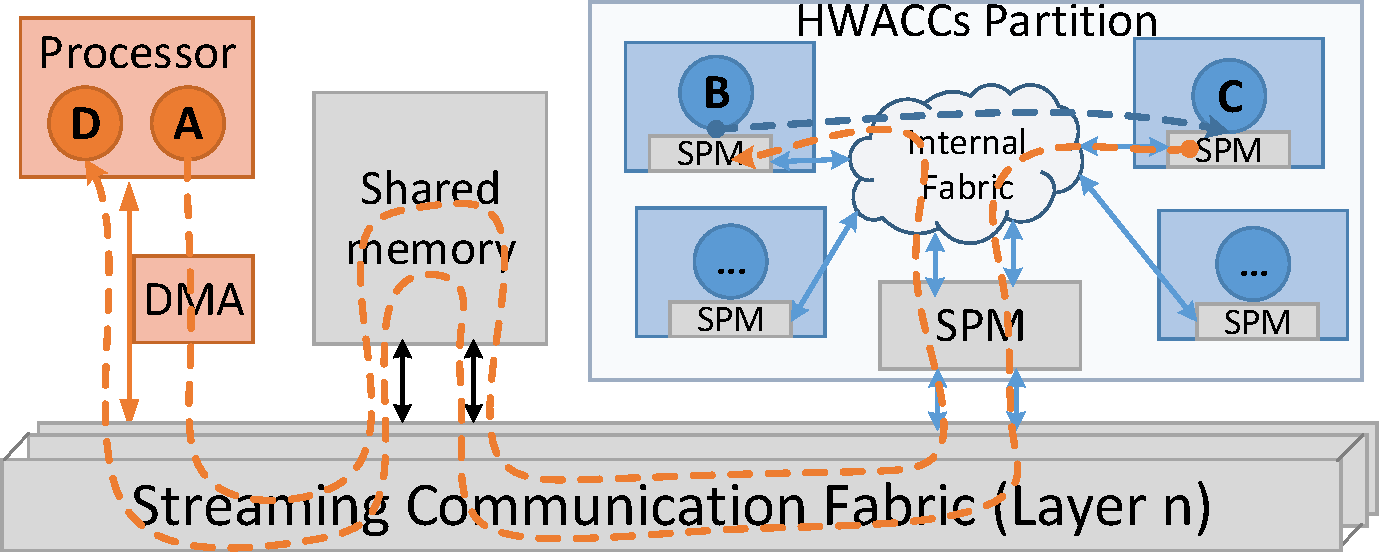
\includegraphics[width=.8\linewidth]{fig/pPlat.pdf}
	\vspace{-4pt}
	\caption{Target Platform}
	\label{fig:plat}
	\vspace{-8pt}
\end{figure}


\vspace{-4pt}
\subsection{Analytic Evaluation}
\label{subsec:ana}

Evaluating performance follows a speed/accuracy trade-off.
A vast number of evaluation is needed due to (a) the enormous domain design space which needs to be traversed (b) the number of applications which must be evaluated for each allocation. 
An abstract and dramatically fast evaluation, analytic evaluation, is desired to evaluate many more points at the cost of accuracy.

%\begin{figure}[h]
%	\centering
%	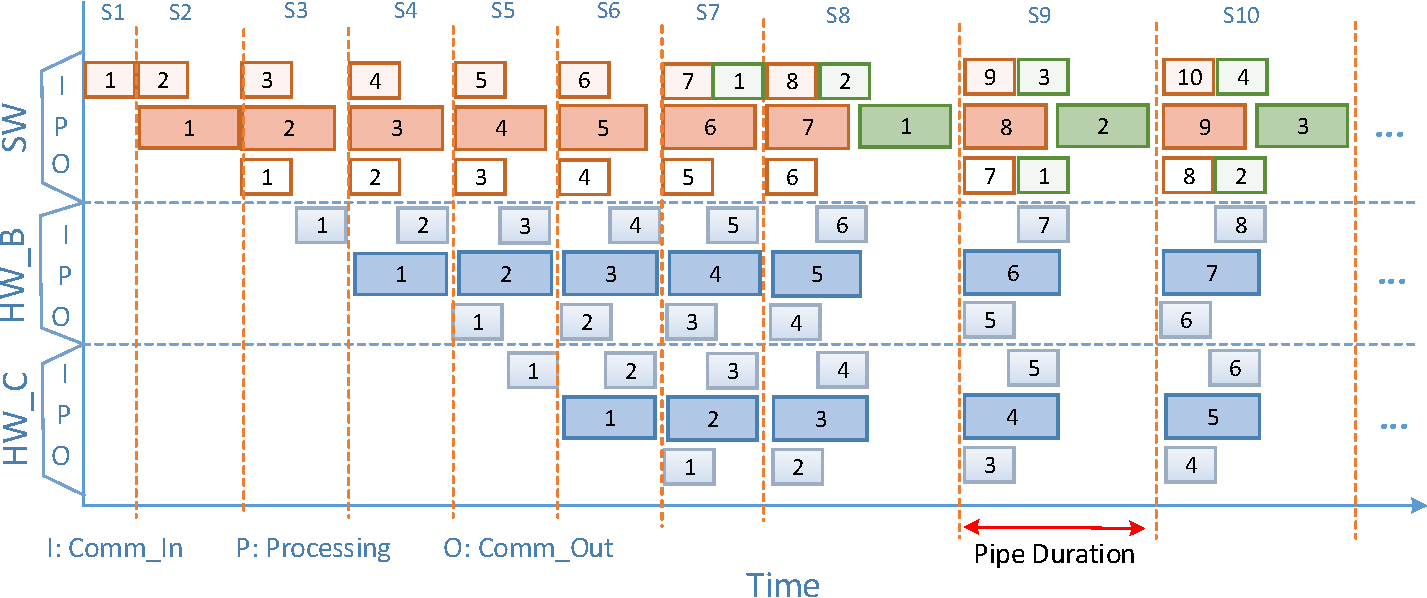
\includegraphics[width=\linewidth]{fig/pPipe.pdf}
%	\caption{Timing diagram of Architecture}
%	\label{fig:Pipe}
%\end{figure}

\newtext{
We incorporate the analytic model~\cite{Teimouri_TCAD_2018} to do the fast evaluation. 
In the analytic model, the kernels in a streaming application operate as producers and consumers of the streaming data and form a pipeline. 
Each pipe stage overlaps communication (in/out) with processing due to double buffering. Actors execute concurrently given their dependencies across different processing components. Actors mapped to the same component execute sequentially.
Our Analytic Evaluation model computes the throughput ($Th$) of an application based on the inter-kernel pipelined execution.
At this abstraction, the throughput only depends on the pipe latency ($L$) which is determined by the slowest processing component (or communication).
The model also records energy consumption ($EC$) for processing, data transfer, and memory.
We validated the accuracy of the analytical model against SCE \cite{SCE} generated virtual platforms. On a set of 100 different platform allocations, the application performance fidelity achieved 98\%.
}
